%%%%%%%%%%%%%%%%%%%%%%%%%%%%%%%%%%%%%%%%%%%%%%
%% Created by John Paul Minda, PhD			%%
%% Professor of Psychology					%%
%% The Brain and Mind Institute				%%
%% The University of Western Ontario		%%	
%% London, ON N6A 5C2						%%
%%											%%
%% Version 1.2								%%	
%% Feb 13, 2018								%%
%%%%%%%%%%%%%%%%%%%%%%%%%%%%%%%%%%%%%%%%%%%%%%

\documentclass{article}
\usepackage{fullpage}

\renewcommand{\familydefault}{\sfdefault}
\usepackage[scaled=1]{helvet}
\usepackage[helvet]{sfmath}
\everymath={\sf}

\usepackage{parskip}
\usepackage[colorinlistoftodos]{todonotes}
\usepackage[colorlinks=true, allcolors=blue]{hyperref}
\usepackage{lipsum}
\usepackage[svgnames]{xcolor}
\usepackage[tikz]{bclogo}
\usepackage{mdframed}
\usepackage{graphicx}
\usepackage{float} 
\newenvironment{important}[1][]{%
   \begin{mdframed}[%
      backgroundcolor={yellow!15}, hidealllines=true,
      skipabove=0.7\baselineskip, skipbelow=0.7\baselineskip,
      splitbottomskip=2pt, splittopskip=4pt, #1]%
   \makebox[0pt]{% ignore the withd of !
      \smash{% ignor the height of !
         \fontsize{20pt}{20pt}\selectfont% make the ! bigger
         \hspace*{-19pt}% move ! to the left
         \raisebox{0pt}{% move ! up a little
            {\color{yellow!100!white}\sffamily\bfseries 
\includegraphics[height=\fontcharht\font`\B]{J6520}}% type the bold red !
         }%
      }%
   }%
}{\end{mdframed}}

\newenvironment{note}[1][]{%
   \begin{mdframed}[%
      backgroundcolor={blue!15}, hidealllines=true,
      skipabove=0.7\baselineskip, skipbelow=0.7\baselineskip,
      splitbottomskip=2pt, splittopskip=4pt, #1]%
   \makebox[0pt]{% ignore the withd of !
      \smash{% ignor the height of !
         \fontsize{20pt}{20pt}\selectfont% make the ! bigger
         \hspace*{-19pt}% move ! to the left
         \raisebox{0pt}{% move ! up a little
            {\color{blue!100!white}\sffamily\bfseries 
\includegraphics[height=\fontcharht\font`\B]{note2}}% type the bold red !
         }%
      }%
   }%
}{\end{mdframed}}

\title{Westcott 12" Paper Trimmer User Instructions}
\author{Gabriel Mauger, Ziad Arafat}
%\company{The University of Western Ontario}
\setcounter{tocdepth}{2}
\begin{document}
\maketitle
\tableofcontents

\section{Introduction} 
The following instructions are meant to teach the reader how to use the Westcott 12” Plastic Paper Trimmer, including how to load paper onto the paper-trimmer, how to slice the paper using the paper-trimmer, and how to resolve some common issues that arise while using the paper-trimmer.
\begin{important}
 This product contains two sharp blades that, if mishandled, can cause potential injury to the user.
\end{important}




\subsection{About the Westcott 12" Paper Trimmer}

The Westcott 12” Plastic Paper Trimmer is a standard office item used to make straight cuts across several pieces of paper at one time. This is helpful in a variety of ways, from cutting large pieces of paper into smaller flashcards to trimming the irregular edges off of scrap paper for crafts.

\subsection{terminology}
\begin{itemize}
    \item \textbf{Table}
        \begin{itemize}
        \item The surface of the trimmer where papers are placed.
        \end{itemize}
    \item \textbf{Ruler}
        \begin{itemize}
        \item The blue plastic piece which folds up and down to clamp over the papers. Used to measure length of trims.
        \end{itemize}
    \item \textbf{Scaleline} Guide
        \begin{itemize}
        \item these are the marked rules on either side of the trimmer used to measure depth of trims.
        \end{itemize}
    \item Blade Holder (Cartridge)
        \begin{itemize}
        \item This is the small cube-shaped widget which contains the blades.
        \begin{important}
         Blade cartridge is extremely sharp. To avoid injury keep fingers out of blade cartridge.
        \end{important}
        \end{itemize}

    \item Blade
        \begin{itemize}
        \item The blade inside of the holder can be identified as a small metal nub.
        \end{itemize}
    \item Grid
        \begin{itemize}
        \item A section of the \textbf{Table} is lined with a grid pattern. Each square of the grid is half an inch by half an inch.
        \end{itemize}
    \item Angle Guides
        \begin{itemize}
        \item Over the grid there are diagonal lines which can be used to measure the angle of trims.
        \end{itemize}
    \item Blade Track
        \begin{itemize}
        \item The blade track is a crease on the edge of the table where the ruler aligns. The blade holder slides along this track to trim the papers.
        \end{itemize}
\end{itemize}

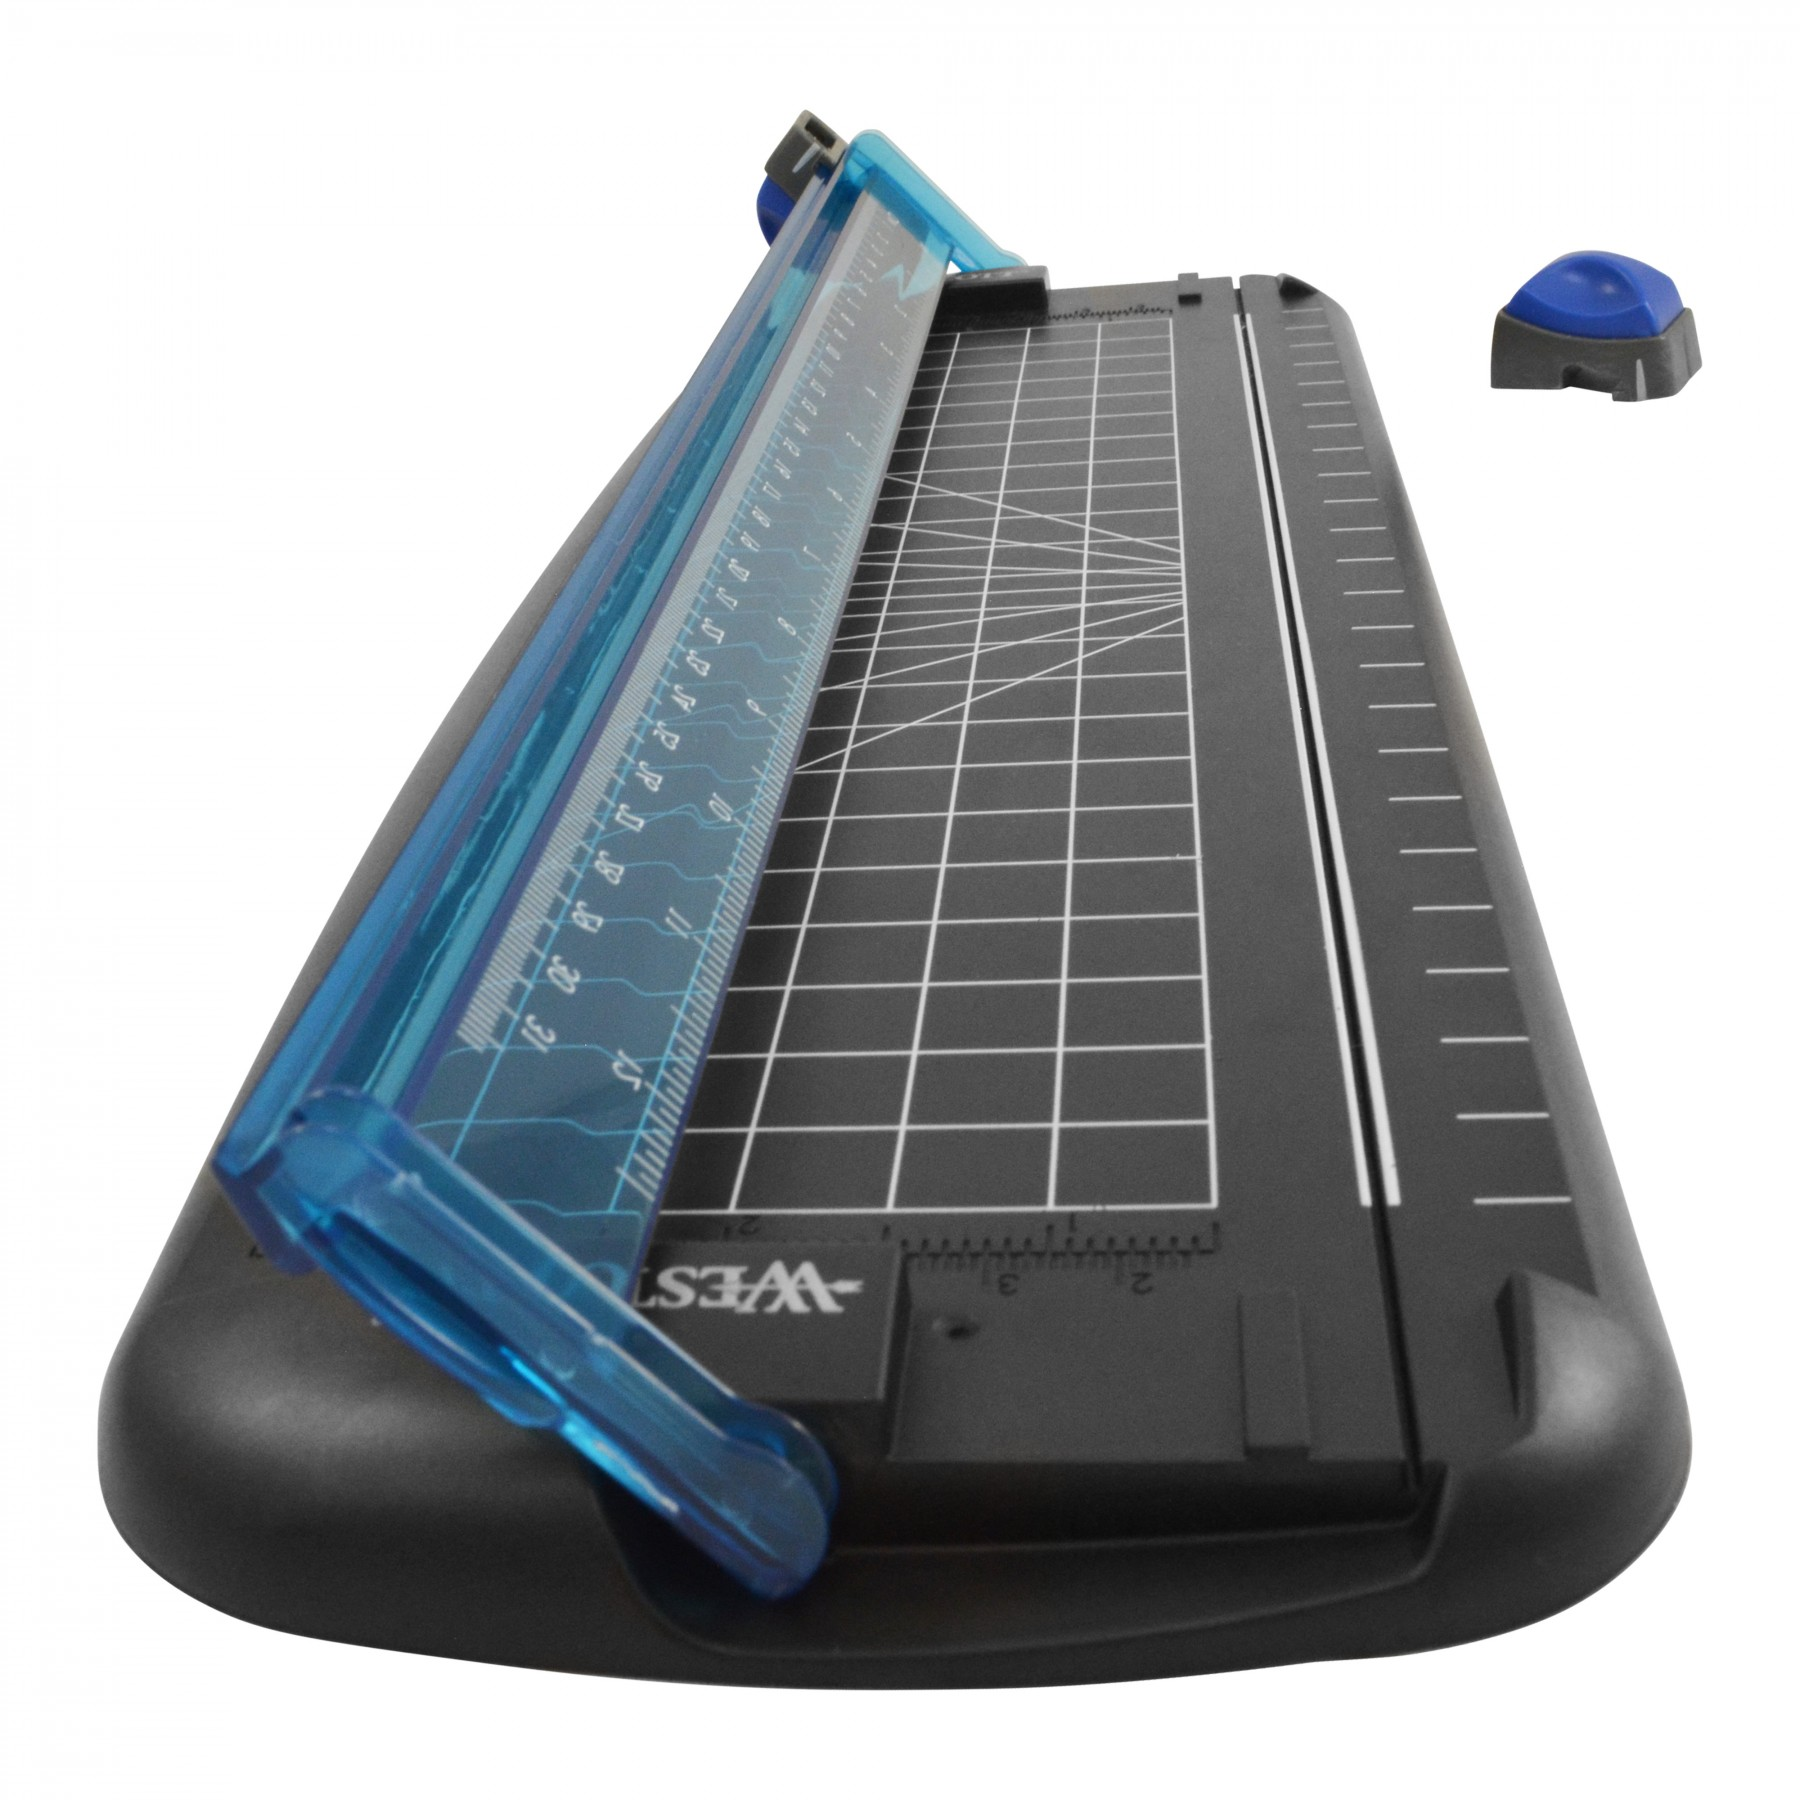
\includegraphics[height=200pt]{trimmer0.jpg}

\subsection{Principle of Operation}

The Westcott Paper Trimmer slices through paper using two blades located under the Blade Holders, two plastic buttons that slide along the \textbf{Ruler}. A small stack of paper is placed on the \textbf{Table} - the base of the paper cutter - and under the \textbf{Ruler}.  Once the paper is aligned against the desired \textbf{Scaleline} Guide, Grid Line or Angle Guideline (located on the \textbf{Table}), the user presses down on one Blade Holder and slides it across the \textbf{ruler}; this effectively extends the blade into the paper and slices through it in a straight line. If some of the paper remains uncut, the process is repeated with the second Blade Holder.
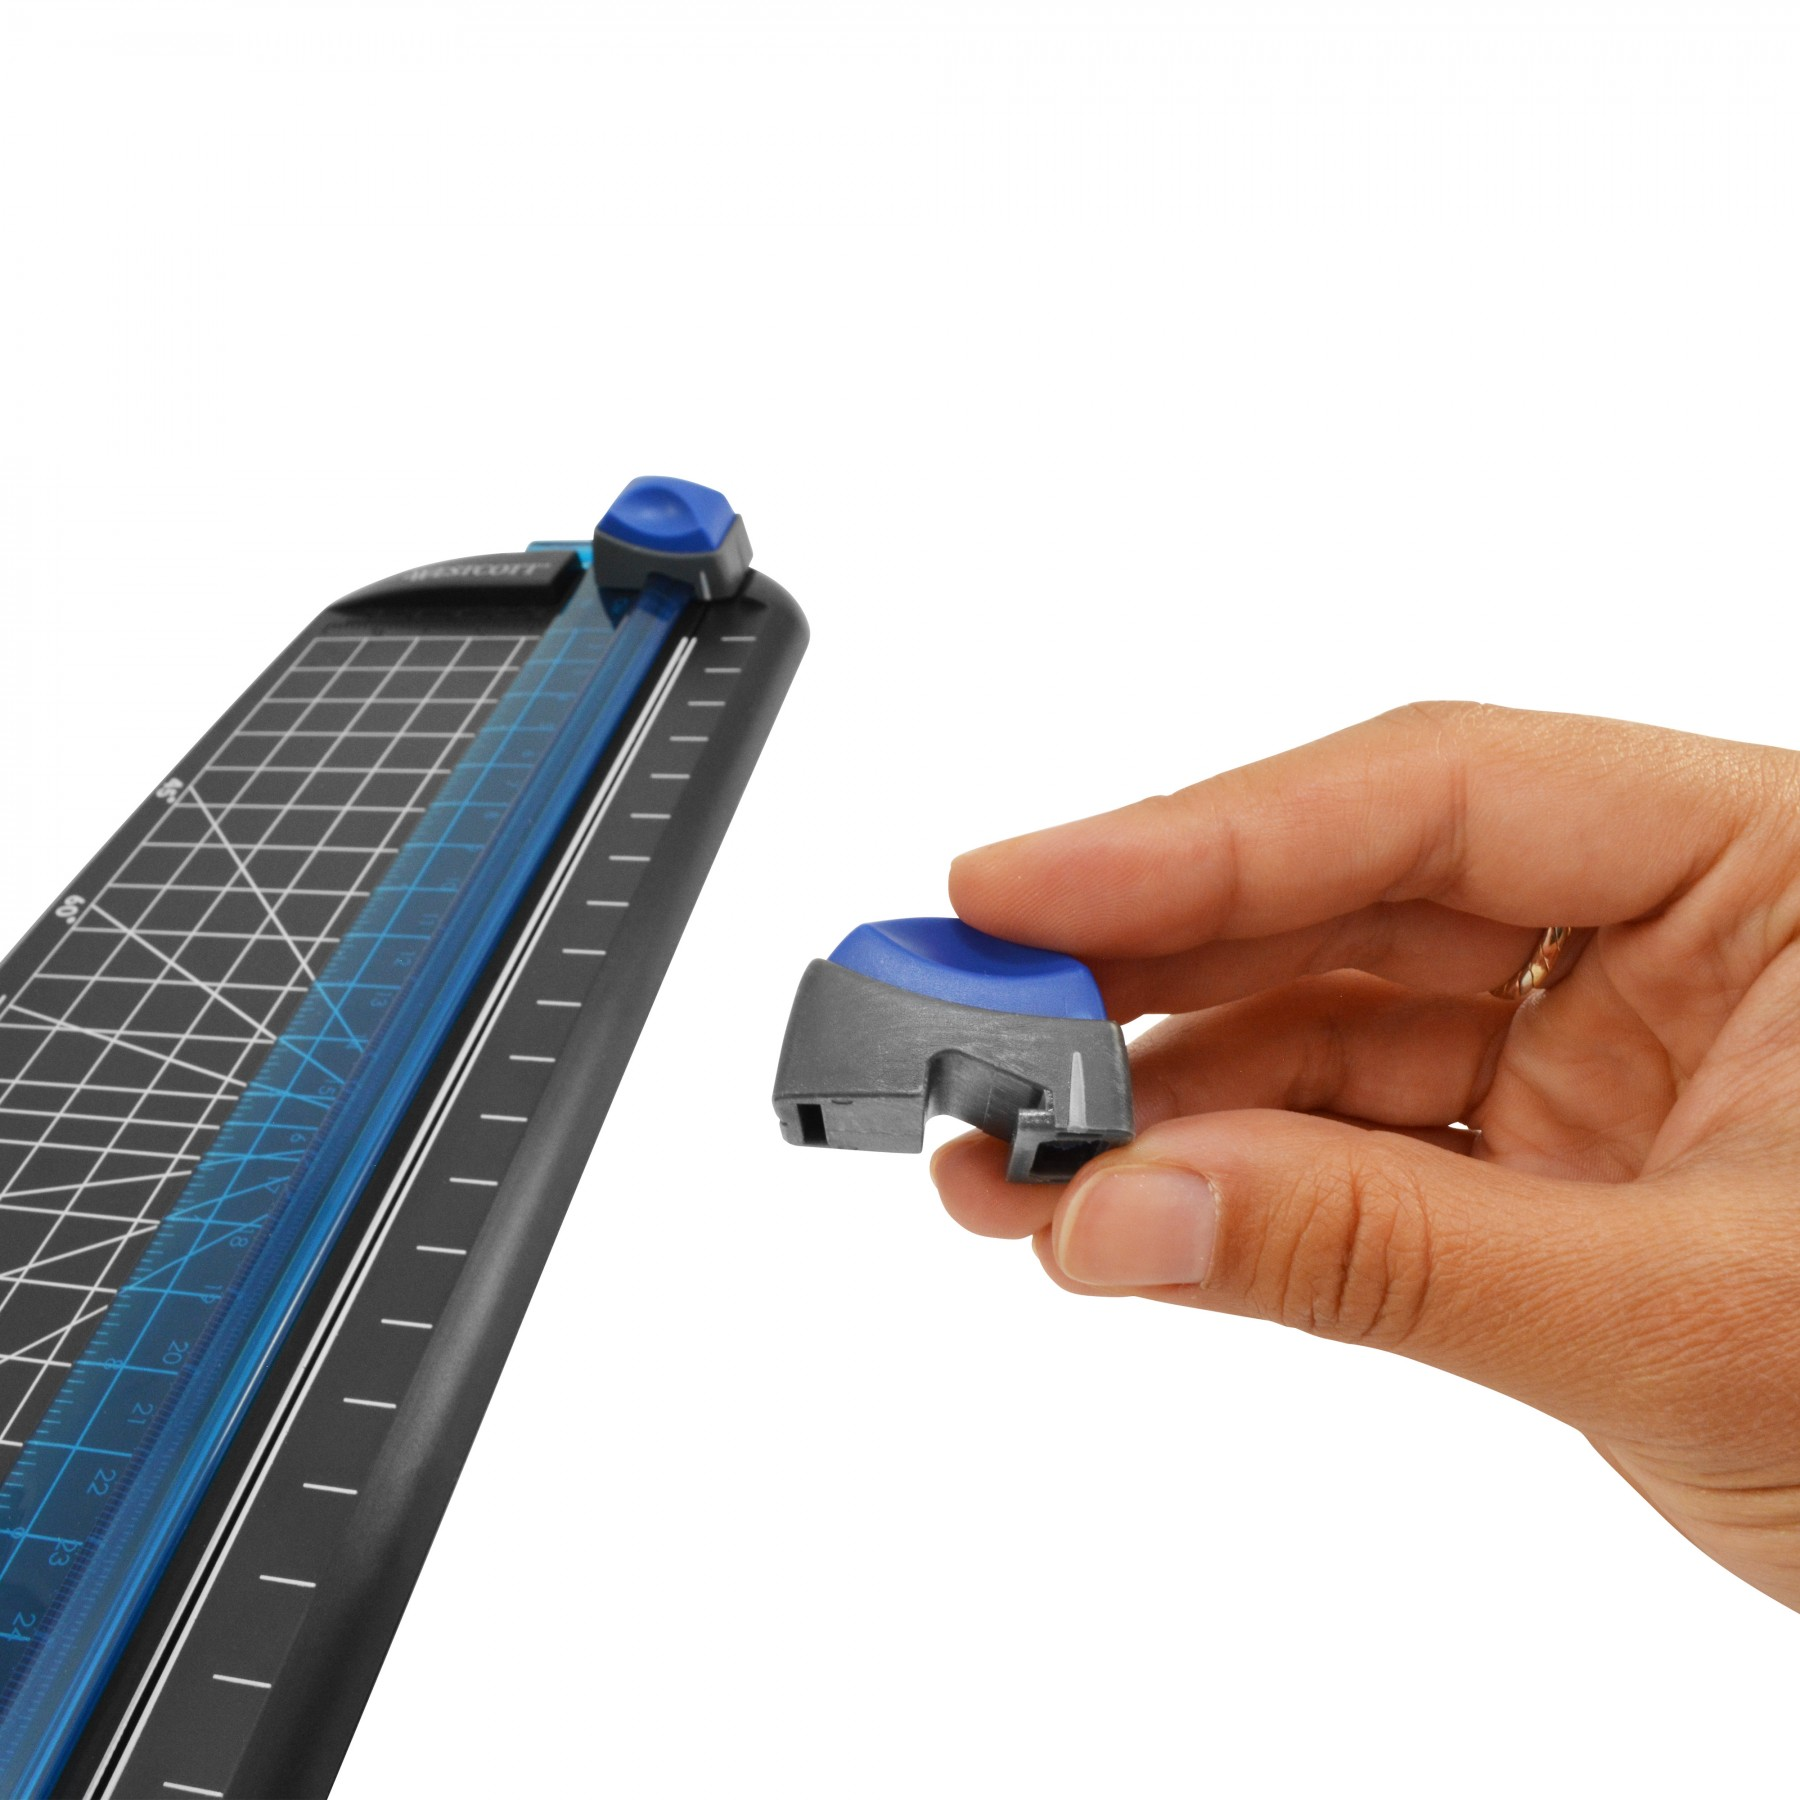
\includegraphics[height=200pt]{trimmer1.jpg}

\section{Usage}

\subsection{Setup}

\begin{enumerate}

    \item If the Paper Trimmer was used before, remove any excess paper from the Blade Track.
    \item Make sure both Blade Holders are moved all the way to one side of the \textbf{ruler}.
    \item Take the paper that is to be cut (10 pages at the most) and make certain the edges of the pages are aligned.
\begin{note}
    Step 3 can be skipped if scrap paper is used
\end{note}
    
\end{enumerate}




\subsection{Using the paper trimmer}

\begin{enumerate}
    \item Lift the \textbf{Ruler} to the “up” position.
    \item Place the prepared paper on the Westcott \textbf{Table}, sliding it underneath the \textbf{Ruler}
    \item Align the paper against the preferred Grid Line or Angle Guideline. Use the \textbf{Scaleline} Guide to choose the desired width of the cut paper.
    \item Lower the \textbf{Ruler} to the “down” position, ensuring that both Blade Holders are still all the way to one side.
    \item Press down on the innermost Blade Holder.
    \item Slide the Blade Holder all the way to the other side of the \textbf{Ruler}.
\begin{important}
 Stop immediately if there is too much resistance, for this may damage the product. If this occurs, check for excessive debris or remove several pieces of paper until the Blade Holder glides easily across
\end{important}
    
    \item Lift the \textbf{Ruler} and check if the blade cut through all layers of paper on the \textbf{table}.
    \begin{note}
        If some paper remains uncut, repeat step 5 - 6 with the secondary Blade Holder.
    \end{note}
    \item Once all of the paper is cut, remove the paper from the \textbf{table}.

\end{enumerate}
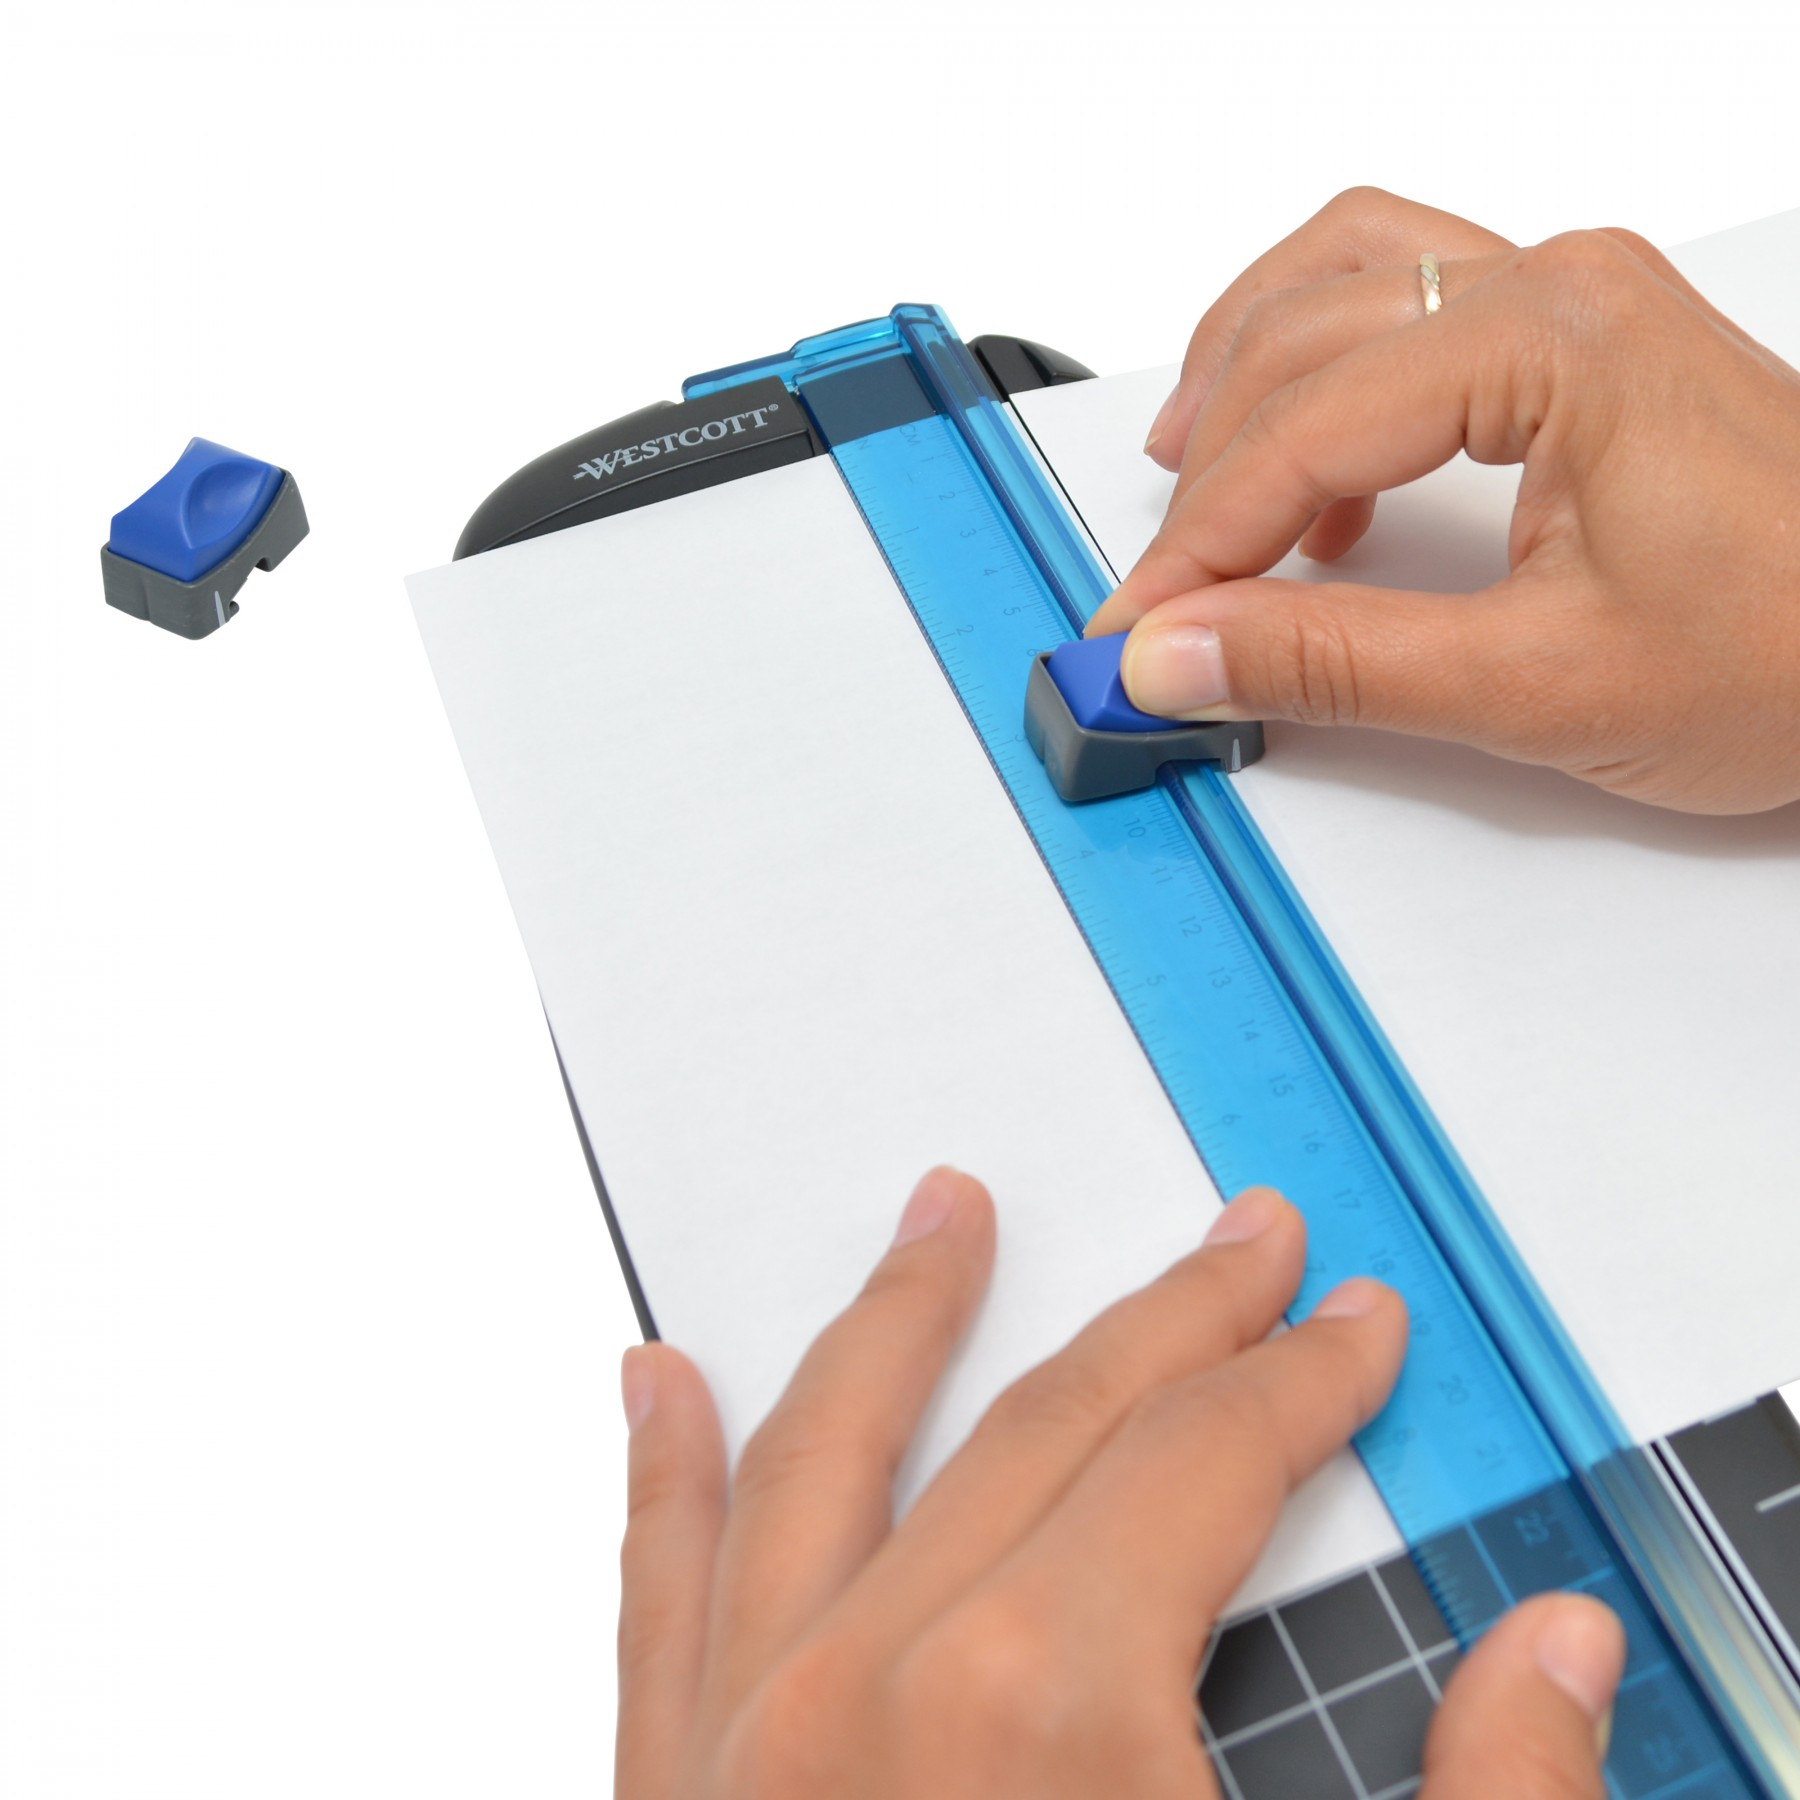
\includegraphics[height=200pt]{trimmer2.jpg}
\subsection{Line Guide Usage}

\begin{table}[H]
\caption{Table Line Guide Usage}
\label{my-label}
\begin{tabular}{|l|l|}
\hline
Scale Line Guide & To determine the desired width of the cut piece of paper. \\ \hline
Grid Line Guide  & To check if the paper is parallel                         \\ \hline
Angle Guide      & To cut the paper at a desired angle.                      \\ \hline
\end{tabular}
\end{table}

\section{Troubleshooting}

% Please add the following required packages to your document preamble:
% \usepackage{graphicx}
\begin{table}[H]
\caption{Troubleshooting Sheet}
\resizebox{\textwidth}{!}{%
\begin{tabular}{|l|l|}
\hline
Problem & Solution \\ \hline
Blade is not cutting all of the paper & \begin{tabular}[c]{@{}l@{}}Ensure that the Blade Holders are held down firmly before \\ sliding them across the \textbf{Ruler}.\\ \\ Check if there is any unnecessary debris in the Blade Track.\\ \\ Check if the blades in the Blade Holders are damaged.\\ \\ If the problem continues, remove several pieces of paper \\ before trying again.\end{tabular} \\ \hline
The Blade Holders are stuck & \begin{tabular}[c]{@{}l@{}}Check for debris along the \textbf{Ruler}, in the Blade Track,\\ and underneath the Blade Holders.\end{tabular} \\ \hline
\end{tabular}%
}
\end{table}

\end{document}